\subsection {Collection}
\label{sec:Collection}
The \sbol{Collection} class is a class that groups together a set of \sbol{TopLevel} objects that have something in common.
Some examples of \sbol{Collection} objects:
\begin{itemize}
\item Results of a query to find all \sbol{Component} objects in a repository that function as promoters.
\item A set of \sbol{Component} objects representing a library of genetic logic gates.
\item A ``parts list'' for \sbol{Component} with a complex design, containing both that component and all of the \sbol{Component}, \sbol{Sequence}, and \sbol{Model} objects used to provide its full specification.
\end{itemize}

\begin{figure}[ht]
\begin{center}
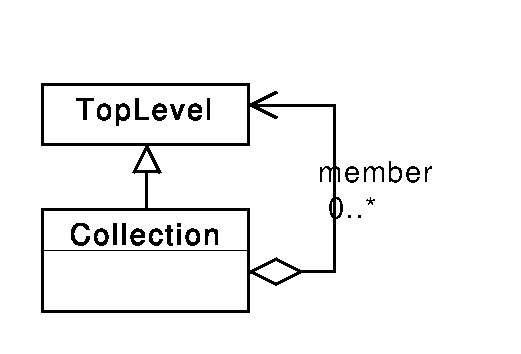
\includegraphics[scale=0.6]{uml/collection}
\caption[]{Diagram of the \sbol{Collection} class and its associated properties.}
\label{uml:collection}
\end{center}
\end{figure}

\subparagraph{The \sbolheading{member} property}\label{sec:member}
A \sbol{Collection} object can have zero or more \sbol{member} properties, each of type \sbol{URI} specifying a \sbol{TopLevel} object.

\subsubsection{Namespace}
\label{sec:Namespace}

The \sbol{Namespace} class is a subclass of \sbol{Collection} and is used to define \sbol{member} entities that share the same URI prefix.  Namely, all linked objects MUST have a URI prefix matching the URI of the \sbol{Namespace} object. 

\subsubsection{Experiment}
\label{sec:Experiment}

The purpose of the \sbol{Experiment} class is to aggregate \sbol{ExperimentalData} objects for subsequent analysis, usually in accordance with an experimental design.  Namely, the \sbol{member} properties of an \sbol{Experiment} MUST refer to \sbol{ExperimentalData} objects.

